\documentclass[12pt]{article}

\usepackage[T1]{fontenc}
\usepackage[utf8]{inputenc}
\usepackage{polski}
\usepackage{amssymb, amsfonts, amsmath}
\usepackage{graphicx}
\usepackage{verbatim}
\usepackage{hyperref}
\usepackage{enumerate}
\usepackage{blindtext}
\usepackage{float}
\begin{document}
\title{Projekt aplikacji do analizy i wizualizacji danych dotyczących wrażeń synestetycznych}
\author{Łukasz Brzozowski}
\maketitle
\begin{figure}[ht!]
	\centering
	
\includegraphics[width=\textwidth]{MiNI.png}
\end{figure}
\begin{figure}[ht!]
	\centering
	
\includegraphics[width=8cm]{Pw.png}
\end{figure}
\pagebreak
\section{Opis problemu}
	Celem projektu jest stworzenie aplikacji, która na podstawie danej próbki tekstu będzie dynamicznie tworzyć animacje mające odwzorować wrażenia osób z przypadłością synestezji wzrokowo-leksykalnej. Dzięki takiej aplikacji nastąpi zwiększenie się świadomości społecznej dotyczącej synestezji oraz będzie możliwe przedstawienie codzienności osób z ową cechą. Ponadto, na podstawie danych zebranych od synestetyków zostanie przeprowadzona analiza połączeń kolorystyczno-literowych umożliwiająca odnalezienie najczęstszych wzorców oraz schematów przyporządkowania kolorów.
\begin{figure}[ht!]
	\centering
	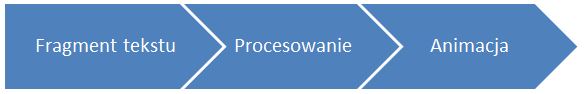
\includegraphics[width=10cm]{Capture.PNG}
	\caption{Działanie aplikacji}
\end{figure} 
\begin{figure}[H]
	\centering
	
\includegraphics[width=\textwidth]{Synesthesia.png}
	\caption{Sposób widzenia liter przez synestetyków wzrokowo-leksykalnych}
\end{figure}
\pagebreak
\section{Analiza istniejących rozwiązań}
Na tę chwilę nie są dostępne żadne narzędzia służące do wizualizacji wrażeń synestetycznych wynikających z powiązań wzrokowo-leksykalnych. Można jednak znaleźć aplikacje animujące wrażenia wzrokowo-słuchowe. Bazują one na indywidualnych skojarzeniach tonacji muzycznych i barw instrumentów z kolorami. 

\subsection{Pokrewny problem}
Jedną z możliwych form wizualizacji jest przyporządkowanie kolorów klawiszom klawiatury fortepianu. Użytkownik serwisu YouTube o nicku aniMIDIfy napisał program w języu Python, korzystając również z oprogramowania FFMPEG, SoX, TiMidity, FluidSynth, Python Image Library oraz midicsv.
\begin{figure}[H]
	\centering
	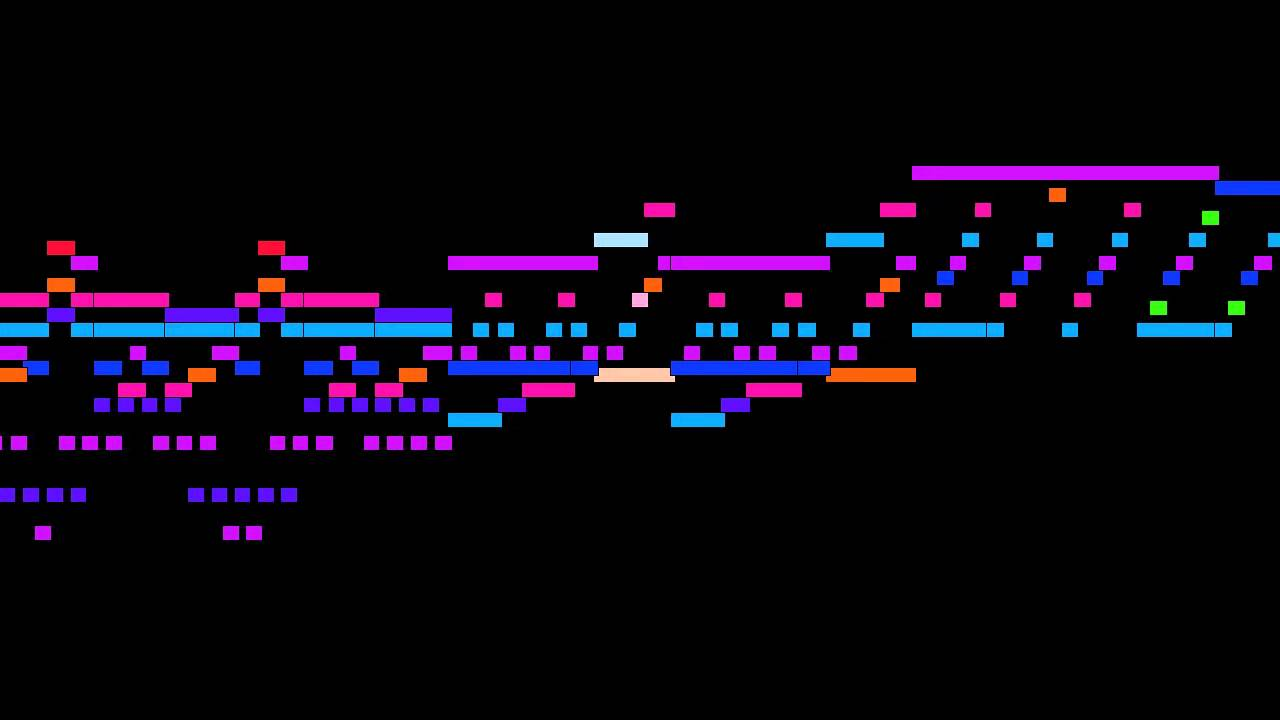
\includegraphics[width=\textwidth]{animidify.jpg}
	\caption{Klatka animacji z jednego z filmów użytkownia aniMIDIfy}
\end{figure}
\section{Wymagania funkcjonalne}
\begin{description}
\item[Algorytm] \hfill \\
\begin{enumerate}
\item{Pobranie próbki tekstu,}
\item{Podzielenie tekstu na litery,}
\item{Stworzenie animacji na bazie utworzonych danych i bazy kolorów,}
\item{Stworzenie suwaka podświetlającego tekst wraz z animacją,}
\item{Stworzenie przycisków "stop", "play".}
\item{Stworzenie interfejsu pozwalającego na wczytanie własnych próbek kolorów}
\end{enumerate}
\item[Prezentacja animacji] \hfill \\
\begin{enumerate}
\item{Wyświetlenie tekstu w dolnej konsoli,}
\item{Wyświetlenie animacji w górnym oknie aplikacji,}
\item{Wyświetlenie suwaka podświetlającego obecnie animowany fragment tekstu,}
\item{Wyświetlenie przycisków "stop", "play".}
\end{enumerate}
\item[Wczytanie własnych próbek kolorystycznych] \hfill \\
\begin{enumerate}
\item{Możliwość przyporządkowania każdej literze i cyfrze koloru na skali RGB}
\item{Wybór poprzez umieszczenie znacznika w wybranym miejscu palety barw}
\end{enumerate}
\end{description}
\section{Wymagania niefunkcjonalne}
\begin{enumerate}
\item{Przejrzysty interfejs,}
\item{Płynne animacje,}
\item{Krótki czas oczekiwania na stworzenie animacji,}
\item{Możliwość szybkiego wczytania nowej próbki tekstu,}
\item{Intuicyjne API.}
\end{enumerate}
\section{Ograniczenia}
\begin{enumerate}
\item{Każdej literze można przyporządkować tylko jeden kolor,}
\item{Jest tylko jeden typ animacji tworzonej przez aplikację,}
\item{Nie ma możliwości przewijania animacji suwakiem wyświetlanym na tekście.}
\end{enumerate}
\section{Interfejs programu}
\begin{figure}[ht!]
	\centering
	\fbox{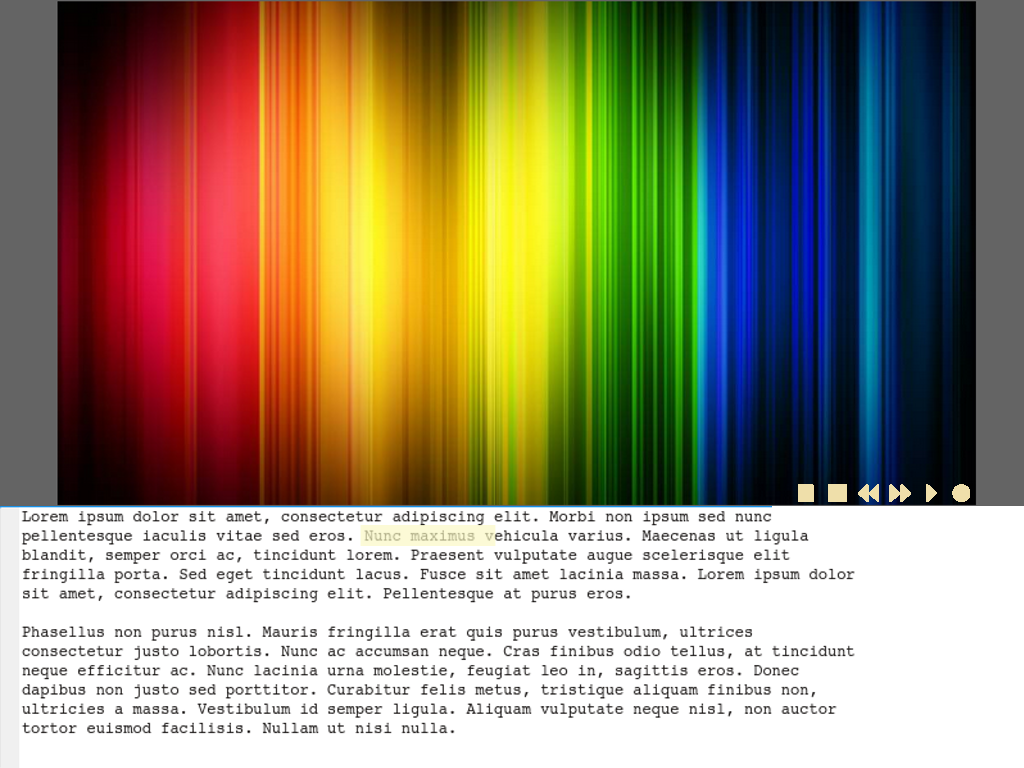
\includegraphics[width=11cm]{Prototyp_programu.png}}
	\caption{Przykładowy interfejs aplikacji dynamicznie tworzącej animacje}
\end{figure}


\end{document}
